\documentclass[preprint2]{aastex}
%manuscript  preprint2
\usepackage{graphicx}
\usepackage{subfigure}
\newcommand{\vdag}{(v)^\dagger}
\newcommand{\myemail}{liujh@smail.nju.edu.cn}
\shorttitle{\objectname{G240} outflow}
\shortauthors{Liu et al.}

\begin{document}
\title{THE ISOTHERMAL OUTFLOW IN HIGH-MASS STAR-FORMING REGION G240.31+0.07}
\author{JUNHAO LIU and KEPING QIU} %\altaffilmark{1}
\affil{School of Astronomy \& Space Science, Nanjing University, Nanjing, P.R.China}
%\email{kpqiu@nju.edu.cn}

\begin{abstract}
We present Atacama Pathfinder Experiment (APEX) observations of the massive star-forming region \objectname{G240.31+0.07} in the CO (3-2), (6-5), and (7-6). The integrated high-velocity and low-velocity emissions of the three lines reveal a bipolar outflow and show similarity in morphology. Together with the combined data from the Submillimeter Array (SMA) and the Caltech Submillimeter Observatory (CSO) 10.4 m telescope in CO (2-1), we explore the physical conditions of the outflowing gas as a function of gas velocity, by the means of Large Velocity Gradient (LVG) modeling and population diagram analysis. Our results reveal that the temperature of the outflowing gas has an almost constant value of $\sim$ 50 K. The constant trend is consistent with the isothermal assumption of the wide-angle wind model. We also find a decreasing trend of CO column density with gas velocity. In addition, the modeling results reveal that the outflowing gas is thermalized and no upper limits to the gas density could be derived. The lower limits of gas density are $n_{\mathrm{low}} \sim 10^5$ cm$^{-3}$ at most velocities.
%T n range. difference with previous. T n relationship . previous 
\end{abstract}

\keywords{ISM:  individual (\objectname{G240.31+0.07}) - ISM: jets and outflows - stars: formation - stars: early-type}

\section{INTRODUCTION}
Bipolar molecular outflows, mostly observed via CO, HCO$^+$ and their isotopes, are a common phenomenon associated with young stellar objects (YSOs) of all masses \citep{2001ApJ...552L.167Z, 2002A&A...383..892B, 2004A&A...426..503W, 2005AJ....129..330W,  2015MNRAS.453..645M}. It is believed that molecular outflows trace the accretion-powered ejections in sites of low-mass star formation. As molecular outflows impact the surrounding material and the parent cloud significantly, they play an important role in the star formation process. Though molecular outflows have been well studied, the driving mechanism of molecular outflows remains unknown. Molecular outflows from low-mass protostars were thought to be entrained by wide-angle winds \citep{1991ApJ...370L..31S, 2001ApJ...557..429L}, or by jet bow shocks \citep{ 1993A&A...278..267R, 1993ApJ...414..230M, 2001ApJ...557..429L}. Though the wind-driven model and the jet-driven model can each explain the characteristics of some observed outflows, none of them are capable of producing the observed features of all types of outflows \citep{2000ApJ...542..925L, 2002ApJ...576..294L}. In order to explain different features of various types of outflows associated with low-mass YSOs simultaneously, two-component models with both highly collimated jet and wide-angle wind have been developed \citep{2000prpl.conf..789S, 2006ApJ...641..949B, 2006MNRAS.365.1131P, 2006ApJ...649..845S, 2007prpl.conf..277P, 2008ApJ...676.1088M}.

Massive molecular outflows are more problematic than their low-mass counterparts. Though observations have shown that the morphology and kinematics of some outflows driven by massive YSOs are very similar to the outflows driven by low mass YSOs \citep[][]{1998ApJ...507..861S, 2002A&A...387..931B, 2009ApJ...696...66Q, 2011MNRAS.415L..49R}, there is a lack of detection of extremely collimated outflows and circumstellar disks towards sources more massive than early B-type YSOs \citep{2007prpl.conf..245A}. Thus, it is not clear whether massive stars form as a scaled-up version of low-mass stars or they form in a different way. Due to the rarity and typically large distances of high-mass YSOs, the sample of individual studies towards outflows driven by massive YSOs is still small. And there is little theoretical work on modeling outflows from high-mass YSOs. Many questions, e.g., how the outflows from massive YSOs are accelerated, how they differ from low-mass outflows, and how they affect the high-mass star-forming processes, are still unanswered. It is essential to address these questions by studying more outflows associated with high-mass star-forming regions. 

Most previous studies of outflows have used low-J rotational transitions of CO (transitions up to J$_u$ = 3, with upper-state energies E$_u$ up to 30 K), which are easily excited at low temperatures, to characterize the relatively cold and extended molecular gas in morphology and kinematics. These low-J CO emission lines can be easily observed from the ground-based facilities. Due to atmospheric limits, mid-J CO lines (referring to CO (6-5) and CO (7-6) throughout this paper, with  E$_u$ up to 150 K), which are less affected by ambient gas, are not commonly observed. In several studies, mid-J CO transitions have been reported to trace the warm gas (T $>$ 50 K) in outflows of low-mass and intermediate-mass YSOs \citep{2009A&A...501..633V, 2009A&A...507.1425V, 2012A&A...542A..86Y, 2016A&A...587A..17V}.  By comparing multi-line CO observations (both low-J and mid-J) with the results of non-LTE radiative transfer models, the physical properties (temperature, density) of the outflowing gas could be well constrained \citep{2015A&A...581A...4L}. 

This paper is a follow-up study of the \objectname{G240.31+0.07} (hereafter \objectname{G240}) outflow \citep{2009ApJ...696...66Q}. We report the 12-m submillimeter Atacama Pathfinder Experiment Telescope\footnote{    The Atacama Pathfinder Experiment Telescope is a collaboration between the Max-Planck-Institut f$\ddot{\mathrm{u}}$r Radioastronomie, the European Southern Observatory, and the Onsala Space Observatory.} (APEX) observations of \objectname{G240}, an active high-mass star-forming region which is associated with the YSO \objectname{IRAS 07427-2400} and located at a distance of 5.41 kpc \citep{2015PASJ...67...69S}. It harbors an ultracompact HII region and is associated with OH and H$_2$O masers \citep{1993AJ....105.1495H, 1997MNRAS.289..203C, 1998AJ....116.1897M, 1999ApJS..123..487M, 2003MNRAS.341..551C}. Its far-infrared luminosity of 10$^{4.7}$ L$_\sun$ is consistent with a spectral type O8.5 zero-age main-sequence star \citep{1998AJ....116.1897M}. \citet{2009ApJ...696...66Q} presented a high resolution interferometric study at 1.3 mm and resolved the central part of \objectname{G240} into three dusty cores MM1, MM2, and MM3. \citet{2003A&A...412..175K} mapped the CO (3-2) emission with a 20${\arcsec}$ beam and found a prominent bipolar outflow at a position angle (PA) of 132${\degr}$ and a weaker component at PA $\sim$ 101${\degr}$. Recently, \citet{2009ApJ...696...66Q} presented a detailed single dish and interferometric study of $^{12}$CO (2-1) and $^{13}$CO (2-1) emissions and detected a bipolar, wide-angle, quasi-parabolic molecular outflow. In addition, \citet{2014ApJ...794L..18Q} reported the detection of an hourglass magnetic field aligned within 20${\degr}$ of the outflow axis.

In this paper, we present a CO multi-transition (2-1, 3-2, 6-5, 7-6) study towards the \objectname{G240} outflow. With rotation diagram (RD) analysis and large velocity gradient (LVG) calculations, we estimate the physical parameters of the outflow as functions of gas velocity. We then discuss the results of the analyses.



\section{OBSERVATIONS}
The Submillimeter Array\footnote{    The Submillimeter Array is a joint project between the Smithsonian Astrophysical Observatory and the Academia Sinica Institute of Astronomy and Astrophysics and is funded by the Smithsonian Institution and the Academia Sinica.} (SMA) observations were carried out on 2008 February 25 with eight antennas in the compact configuration and on 2008 February 16 with seven antennas in the extended configuration. To ensure the coverage of the entire outflow we observed two fields centered at (R.A., del.)$_{J2000}$ = (07$^\textup{h}$44$^\textup{m}$52$^\textup{s}$.49, −24$^\textup{d}$07$^\textup{m}$52$^\textup{s}$.1) and (R.A., del.)$_{J2000}$ = (07$^\textup{h}$44$^\textup{m}$51$^\textup{s}$.07, −24$^\textup{d}$07$^\textup{m}$34$^\textup{s}$.9), respectively. We used Titan as the primary flux calibrator and \object{3c273} as the bandpass calibrator. The time dependent gain was monitored
by observing quasars \object{J0730-116} and \object{J0826-225} every 23 minutes. Visibilities were calibrated using the IDLMIR package and then output to MIRIAD for imaging. With natural weighting the synthesized beams in the compact and extended configurations are about 4${\arcsec}$ $\times$ 3${\arcsec}$ and 1${\arcsec}$.2 $\times$ 1${\arcsec}$, respectively. The shortest baseline in our SMA observations is 16.5 m, corresponding to a spatial scale of 20 ${\arcsec}$ for observations at 225 GHz. Thus, spatial structures more extended than 20 ${\arcsec}$ were not sampled in the SMA observations. This spatial filtering can significantly affect the CO (2-1) maps at velocities close to the cloud velocity. To recover the missing short spacing information we observed the CO (2-1) emission with the Caltech
Submillimeter Observatory\footnote{    The Caltech Submillimeter Observatory was supported by the NSF grant
AST-0229008 and was closed on September 18, 2015.} (CSO) 10.4 m telescope on 2008 February 12. During the observation the weather condition was excellent for 1 mm waveband with $\tau_{225GHz}$ $\approx$ 0.08. The observations were carried out in the on-the-fly mode centered on (R.A., del.)$_{J2000}$ = (07$^\textup{h}$44$^\textup{m}$52$^\textup{s}$.1, −24$^\textup{d}$07$^\textup{m}$49$^\textup{s}$). We obtained a 15 × 15 grid in CO (2-1), with an integration of about 5 s on each cell. The 10${\arcsec}$ cell spacing is about one-third of the CSO beam, which is $\approx$ 32${\arcsec}$.5 in CO (2-1). By observing Mars and Saturn we derived a beam efficiency of 0.58 ± 0.10. The spectrometer used has 1024 channels throughout the 50 MHz bandwidth, resulting in a spectral resolution of 0.0488 MHz (about 0.065 km s$^{-1}$) per channel. The final maps were smoothed to 2 km s$^{-1}$ per channel. The data were reduced using the standard CLASS package. We combined the SMA compact and CSO CO (2-1) data in MIRIAD following a procedure outlined in \citet{1995ApJ...451L..71Z}. 

The 12-m submillimeter Atacama Pathfinder Experiment Telescope\footnote{    APEX is a collaboration between the Max-Planck-Institut f"ur Radioastronomie, the European Southern Observatory, and the Onsala Space Observatory.} (APEX) observations were conducted on . CO (6-5) and CO (7-6) were observed simultaneously. 
\section{Results}
\subsection{CO emission maps}

\begin{figure*}[htbp]
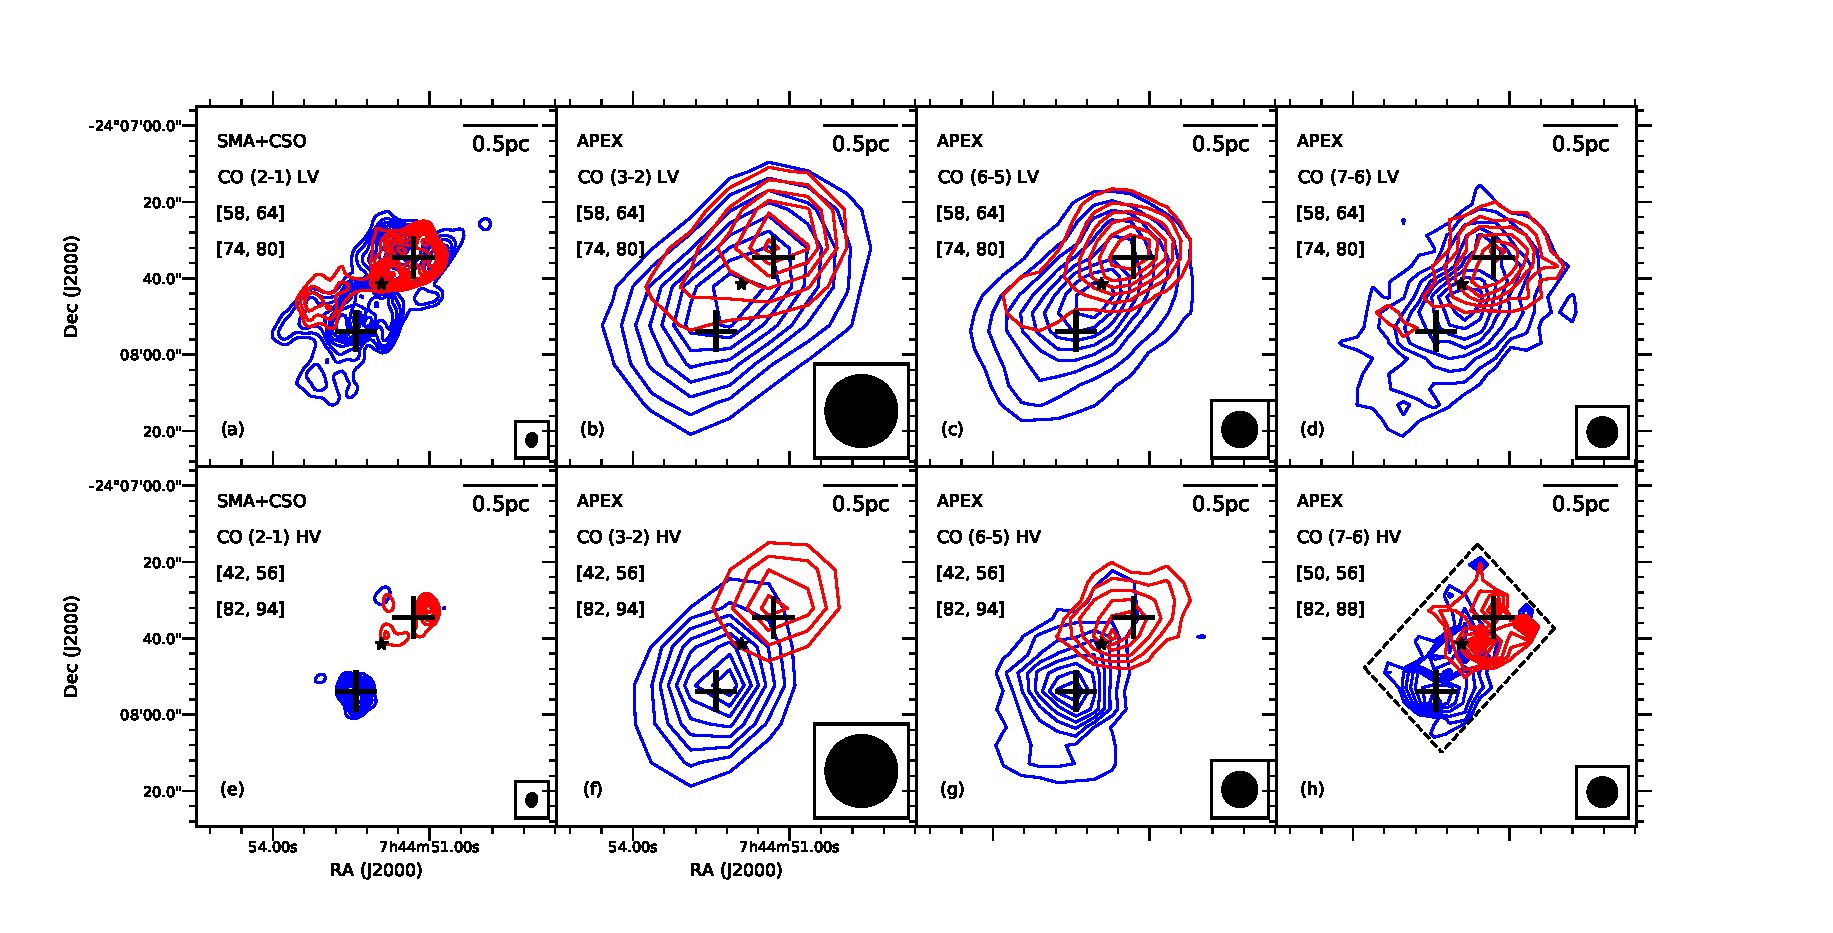
\includegraphics[scale=.65]{./fig/ori_contourall.eps}
\caption{(a)-(d) Low-velocity CO J = 2-1, 3-2, 6-5, 7-6 emissions, integrated from 58 to 64 km s$^{-1} $ for the blueshifted lobe (blue) and from 74 to 80 km s$^{-1}$ for the redshifted lobe (red); (e)-(f) High-velocity CO J = 2-1, 3-2 emissions,  integrated from 42 to 56 km s$^{-1} $ for the blueshifted lobe (blue) and from 82 to 94 km s$^{-1}$ for the redshifted lobe (red); (g) High-velocity CO J = 6-5 emission, integrated from 44 to 56 km s$^{-1} $ for the blueshifted lobe (blue) and from 82 to 92 km s$^{-1}$ for the redshifted lobe (red) (h) High-velocity CO J = 7-6 emission, integrated from 46 to 56 km s$^{-1} $ for the blueshifted lobe (blue) and from 82 to 90 km s$^{-1}$ for the redshifted lobe (red). For (a)-(g), the contour levels start from 20\% and continue at steps of 10\% of the peak emission. For (h), the contour levels start from 30\% and continue at steps of 10\% of the peak emission. Edge channels are masked out because of high noise levels. The black star marks the position of a H$_2$O maser spot which is associated with IRAS 07427-2400 \citep{2015PASJ...67...69S}. The beam of each observational dataset is shown in the lower right corner of each panel. \label{fig:figcontour}}
\end{figure*}

The CO 3-2, 6-5, and 7-6 emissions are detected (with obvious outflow signatures and with peak intensities $>$ 2 $\sigma_{rms}$) in velocity ranges from 42 to 94 km s$^{-1}$, 44 to 92 km s$^{-1}$, and 46 to 90 km s$^{-1}$, respectively. Figure \ref{fig:figcontour} shows the integrated low-velocity (LV) and high-velocity (HV) emissions of the four lines. The velocity ranges chosen to highlight the LV and HV components of the outflowing gas follow those in \citet{2009ApJ...696...66Q}, except that the channels with no detections were excluded for the HV component. The morphologies of the bipolar outflow seen in the CO 3-2, 6-5, and 7-6 lines are very similar. Due to the coarser angular resolutions, the wide-angle structure seen in the higher resolution CO 2-1 image is not seen in the CO 3-2, 6-5, 7-6 maps.

\subsection{Physical conditions of the outflow}
%\subsubsection{Methodology}

\begin{figure}[tbp]
\plotone{./fig/ratio.eps}
\caption{Ratios of the main-beam brightness temperatures of different CO lines at different velocities. Blue symbols denote the measurements from the blueshifted lobe, and red symbols the redshifted lobe. The $V_{\mathrm{outflow}}$ shown here is related to the cloud velocity $v_{\mathrm{cloud}}$ by the relation: $V_{\mathrm{outflow}}$ = $\mid$ $v_{\mathrm{outflow}}$ - $v_{\mathrm{cloud}}\mid$, where $v_{\mathrm{outflow}}$ is the outflow velocity with respect to the local standard of rest. \label{fig:figratio}}
\end{figure}

The physical condition of the outflow can be constrained by comparing the observed line intensities with the results of statistical-equilibrium calculations. To study the four lines at the same spatial resolution, the CO 2-1, 6-5, and 7-6 maps were reconstructed with the same beam of the CO 3-2 map. The rms noise levels are $\sim$0.004 K, $\sim$0.04 K and $\sim$0.1 K for the convolved CO 2-1, 6-5 and 7-6 data, respectively. For both lobes of the outflow, the CO line intensities were measured at approximately the peak positions of the HV components of the convolved CO maps (marked as two crosses in every panel of Figure \ref{fig:figcontour}), and were then used in the following analysis. Figure \ref{fig:figratio} shows the ratios of the main-beam temperatures ($T_{\mathrm{mb}}$) of different CO lines as functions of velocity. The CO 7-6/6-5, 6-5/3-2, and 6-5/2-1 ratios are almost constant over a velocity range of $\sim 5-25$ km s$^{-1}$ with respect to the cloud velocity. In the analysis, we only used channels of $\le$ 60 km s$^{-1}$ and $\ge$ 74 km s$^{-1}$ to avoid contaminations from the ambient gas, and we excluded channels of $<$ 46 km s$^{-1}$ or $>$ 90 km s$^{-1}$ because of their low signal-to-noise ratios. Since we didn't correct the observed line intensities for unknown beam filling factors, the derived CO column densitiy, temperature, and gas density should be considered as beam-averaged values. In the calculation, errors on line intensities took into account both the uncertainties of the flux calibration uncertainty and the rms noise. 
%(R.A., decl.)$_{J2000}$ = ($07^h44^m52^s.4, -24^d7^m53^s.8$) and (R.A., decl.)$_{J2000}$ = ($07^h44^m51^s.3, -24^d7^m34^s.6$)
%We note that the offsets of the peak positions are within $\sim$ 3$\arcsec$ for different lines at different velocities.
%The uncertainty of the observed intensity mainly consists of two parts: the calibration error and the rms noise. At low velocities, the calibration uncertainty dominates the intensity uncertainty, whereas the rms noise is dominant at high velocities. A combination of the rms noise and the calibration error $\sigma_{obs} = (\sigma_{cal}^2 + \sigma_{rms}^2)^{\frac{1}{2}}$ was used as the observational uncertainty in the belowing analyses.
%errors take into account both the rms noise and the calibration uncertainties.

%\subsubsection{Rotation diagram analysis\label{subsec:RD}}

\begin{figure}[tbp]
\plotone{./fig/RD.eps}
\caption{A rotation diagram for CO at 84 km s$^{-1}$. The fitted line shows the Boltzmann distribution of the rotational populations. The line represents a rotational temperature of 48.5 K and a total column density of 2.0 $\times$ 10$^{15}$ cm$^{-2}$. The black solid circles show the data with error bars. \label{fig:figrd}}
\end{figure}

We first performed a simple rotation diagram (RD) analysis \citep{1999ApJ...517..209G} to estimate the excitation condition of the outflowing gas under the assumption of local thermal equilibrium (LTE). Considering that the $^{13}$CO 2-1 emission was only marginally detected at 60 km s$^{-1}$ and 78 km s$^{-1}$ \citep{2009ApJ...696...66Q}, we assumed the four $^{12}$CO lines to be optically thin at our considered velocities. The population of each energy level is given by 
\begin{equation}
N_{\mathrm{up}} = \frac{N_\mathrm{CO}}{Z} g_\mathrm{up} e^{-E_\mathrm{up}/kT_\mathrm{kin}},
\end{equation}
where $N_\mathrm{up}$ is the column density in the upper state, $g_\mathrm{up}$ the statistical weight of the upper state, $E_\mathrm{up}$ the upper energy level, $k$ the Boltzmann constant, and $Z$ is the partition function. The rotation diagram for CO at 84 km s$^{-1}$ is shown in Figure \ref{fig:figrd} as an example. An LTE model at 48.5 K could account for the measurements from the four lines. Other velocity channels show similar rotation diagrams.

%\subsubsection{Large velocity gradient analysis\label{subsec:LVG}}

\begin{figure*}[!tbp]
\gridline{\fig{./fig/chiimage_nco_paper.eps}{0.5\textwidth}{(a)}
        \fig{./fig/chiimage_nh2_paper.eps}{0.5\textwidth}{(b)}}
 \gridline{\fig{./fig/chiimage_tkin_paper.eps}{0.5\textwidth}{(c)}
      }
\caption{(a)-(c) The $\chi^2$ distribution at 84 km s$^{-1}$ in the [$T$, $n$], [$T$, $N$] and [$n$, $N$] planes, with the third parameter fixed to the value of the best fitting result at this velocity. The lower limit of gas density is 1.8 $\times$ 10$^{5}$ cm$^{-3}$. The best-fit solution is obtained for $T$ =  46.1 K and $N$ = 2.2 $\times$ 10$^{15}$ cm$^{-2}$. The $\chi^2_{\mathrm{red}}$ of the best-fit solution is 1.00. The Solid white contours show the 1$\sigma$ confidence levels. \label{fig:figchi}}
\end{figure*}

To better constrain the gas temperature ($T$), the density ($n$), and the CO column density ($N$) without assuming LTE and optical thin emission, we then performed radiative transfer calculations of the four lines using the RADEX code, which adopts the LVG approximation \citep{2007A&A...468..627V}. We built a large grid of LVG models by varying the three parameters ($n$, $T$ and $N$), and obtained the best fitting results by $\chi^2$ minimization in comparing the observation with the models. With four lines observed and three parameters to constrain, our fitting had one degree of freedom. In Figure \ref{fig:figchi}, the fitting results at 84 km s$^{-1}$ are shown. Figure \ref{fig:figchi}(a) and Figure \ref{fig:figchi}(b) show that the gas temperature is well constrained to $sim$ 50 K. In Figures \ref{fig:figchi}(b) and \ref{fig:figchi}(c), the CO column density is stringently constrained to 2.2 $\times$ 10$^{15}$ cm$^{-2}$. The $\chi^2$ distribution in Figure \ref{fig:figchi}(a) and \ref{fig:figchi}(c) indicate that in the best LVG models, the gas density is high enough to thermalize the emissions, and thus only lower limits of the gas density could be derived from the $\chi^2$ minimization. This implies that the LTE assumption adopted by the above RD analysis is valid, and hence we obtain similar gas temperatures and CO column densities from the RD and LVG analyses. Similar $\chi^2$ distribution patterns were found at other velocities. The reduced $\chi^2$ ($\chi^2_{\mathrm{red}}$) of the best fitting results varies from 0.10 to 1.72 at different velocities. The representative uncertainty of each parameter is derived from the 1$\sigma$ confidence region in the 3D parameter space at the velocities where $\chi^2_{\mathrm{red}} \sim 1$: the relative uncertainty of the CO column density is $\sim$ 10 \%; the temperature is found in the range of about 40 - 60 K; and the gas density is $>$ 10$^5$ cm$^{-3}$ over the velocity range. The modeling results also predict that the four transitions are optically thin in the outflowing gas. Figure \ref{fig:figsed} shows the comparison of the observed CO intensities with the LVG modeling results in each velocity bin. 
% Though the best-fitted $\chi^2_{\mathrm{red}}$ varies, the $\chi^2_{\mathrm{red}}$ distribution profiles show similarity in morphology at different velocities, indicating that the uncertainties of the fitted parameters may have similar levels at different velocities.

%\subsubsection{$T$-$V$ and $N$-$V$ relations}

\begin{figure*}[!tbp]
\gridline{\fig{./fig/tv_paper.eps}{0.5\textwidth}{(a)}
          \fig{./fig/Nv_paper.eps}{0.5\textwidth}{(b)}
          }
\caption{$T$-$V$ and $N$-$V$ diagrams of the G240 outflow, estimated from the rotation diagram analysis (blue ``x'' markers for the blue lobe and red ``x'' markers for the red lobe) and the LVG analysis (blue open squares for the blue lobe and red open squares for the red lobe). \label{fig:figrelation}}
\end{figure*}

The variation of the physical conditions of the outflowing gas as a function of velocity is of great interests to our understanding of the driving mechanism of the outflow. With the RD and LVG analyses we have estimated the gas temperature, density and CO column density at different velocities. Figure \ref{fig:figrelation} shows the temperature-velocity ($T$-$V$) and CO column density-velocity ($N$-$V$) relations. We performed RD and LVG analyses of the CO lines in different positions, and obtained similar $T$-$V$ and $N$-$V$ relations.
%In Figure \ref{fig:figrelation}, the $T$-$V$ diagram shows that the gas is approximately isothermal with a gas temperature of $\sim$ 50 K, while the $N$-$V$ diagram shows that the CO column density in each 2 km s$^{-1}$ bin decreases from $\sim 2 \times 10^{16} $ cm$^{-2}$ at $\sim \pm$ 7 km s$^{-1}$ down to $\sim 4 \times 10^{14}$ cm$^{-2}$ at $\sim \pm$ 22 km s$^{-1}$. We compared the model intensities with line intensities measured at several different positions, and found that the modeling results are similar to those represented in Figure \ref{fig:figrelation}. Thus, a systematic bias of position offsets was excluded.
%Thus, we exclude the systematic bias from choices of positions for measuring the line intensities.





\section{DISCUSSION}\label{discussion}
Since the molecular outflow from YSOs was discovered, several outflow models on explaining how outflows are driven have been proposed \citep{2007prpl.conf..245A}. Among these models, the wide-angle wind-driven model \citep{1991ApJ...370L..31S,1996ApJ...472..211L, 2001ApJ...557..429L} and the jet-driven bow shock model \citep{ 1993A&A...278..267R, 1993ApJ...414..230M, 2001ApJ...557..429L} have been proven to be the most promising models.
In the wind-driven model, a molecular outflow is the ambient material swept-up by a wide-angle radial wind. In the jet-driven bow shock model, a molecular outflow is accelarated by a jet bow shock when a jet propagates into the ambient gas.

\subsection{Temperature}


The $T-V$ relation of outflows have been studied by several authors.  A rising CO 3-2/6-5 ratio is observed towards the outflow associated with low-mass YSO HH 46 IRS 1\citep{2009A&A...501..633V}. With the density assumed to be constant, the rising ratios at more extreme velocities correspond to lower kinetic temperatures. In the case of the outflow associated with low-mass protostars NGC 1333 IRAS 4A and  IRAS 4B, the CO 3-2/6-5 ratios are remarkably constant with velocity \citep{2012A&A...542A..86Y}. With the assumption of constant density, the constant ratios indicate constant temperatures. \citet{2012ApJ...744L..26S} have imaged the extremely high velocity (EHV) outflow in CO (2-1) and CO (3-2) associated with the high-mass YSO G5.89-0.39. With the assumption of a canonical CO fractional abundance of 10$^{-4}$, an increasing trend of temperature with outflow velocity is found by performing a LVG analysis. Using the CO (6-5), (7-6) and (16-15) lines, \citet{2015A&A...584A..70L} performed a RD analysis towards the G5.89-0.39 outflow and found a decreasing trend of temperature with increasing velocities. This disagreement seen in results of \citet{2012ApJ...744L..26S} and \citet{2015A&A...584A..70L} could be due to different angular resolutions (3${\arcsec}$.4 compared to 14${\arcsec}$.5 ). The different $T-V$ relations found in different outflows and in different angular scales reveal the complexity of molecular outflows. However, with only two or three lines observed, their derived $T-V$ relations must be deduced from priori assumptions of other physical parameters, e.g., constant density or canonical CO fractional abundance, or from theoretical considerations, e.g., LTE. To get more proper estimations of the pysical parameters of the molecular outflow, multi-line studies of CO are needed.

The LVG analysis and the RD analysis reveal that the G240 outflow is isothermal and has a temperature of $\sim$ 50 K . This value is consistent with temperatures in excess of 50 K probed by \citet{2016A&A...587A..17V} for outflows associated with intermediate-mass protostars, and slightly lower than temperatures of outflows associated with low-mass protostars \citep{2009A&A...501..633V, 2012A&A...542A..86Y}. The isothermal state rules out the jet-driven bow shock models, which predicts temperature rising with outflow velocity and distance, and provides evidence for the wind-driven model \citep{2007prpl.conf..245A}. As molecular cooling dominates the cooling of the shocked material in the outflow at temperatures below 10$^4$ K \citep{1997IAUS..182..181H} and the cooling rate increases as $n^2$, molecular cooling is very efficient for the density of a wind-driven outflow. Thus, an isothermal state could be reached in a wind-driven outflow. We noticed that there are faint bow-shaped H$_{2}$ features near the YSO \objectname{IRAS 07427-2400}, suggesting that the jet-driven outflows may also exist. However, as the average T-V relation of the outflowing gas agrees with the wind-driven model and the kinematics and morphology of the molecular outflow can also be qualitatively interpreted by the wide-angle wind-driven model \citep{2009ApJ...696...66Q}, we conclude that even if the jet-driven outflows and the wind-driven outflows were co-existing in the G240 outflow, the wide-angle wind entrainment plays a more important role in driving the G240 outflow. It should be noted that, most existing outflow models have parameters typical of low-mass outflows. It is necessary to compare the observational results of high-mass outflows with models of similar physical conditions. Statics of outflows associated with high-mass star-forming regions are also essential for us to better understand the driven mechanism of massive outflows and the forming process of high-mass stars.

\subsection{Density}

The LVG analysis reveals that the lower limits of gas densities are $\sim 10^5$ cm$^{-3}$ at the velocities where $\chi^2_{\mathrm{red}} \sim 1$. We have found a decreasing trend of the beam averaged CO column density with gas velocity. As shown in the $N$-$V$ diagram of Figure \ref{fig:fig4}, for each velocity bin (2 km s$^{-1}$), the beam averaged CO column density drops from $\sim 2 \times  10^{16} $ cm$^{-2}$ to $\sim 8 \times 10^{14}$ cm$^{-2}$ within 15 km s$^{-1}$. In the optically thin case, the beam averaged CO column density could be related to gas density $n_{\mathrm{H}_2}$: 
\begin{equation}
N_{\mathrm{CO}} = n_{\mathrm{H}_2} \times \Delta V \times \frac{1}{dv/dr} \times X_{\mathrm{CO}} \times f_{\mathrm{b}}, 
\end{equation}
where $f_{\mathrm{b}}$ is the beam filling factor, $X_{\mathrm{CO}}$ the CO/H$_2$ abundance ratio, $\Delta V$ the velocity interval and $dv/dr$ is the velocity gradient. A drop in $N_{\mathrm{CO}}$ at more extreme velocities indicates the decrease of one or serveral of these parameters. 
To explore how the effect of beam dilution influence our results, we vary the beam filling factors from 0.2 to 1 and then perform the LVG analysis again. We find that modelling with different beam filling factors mainly affect the $N$-$V$ diagram, with minor change in the $T$-$V$ diagram and density limits. This could be resulted from the degeneracies of the beam filling factor with CO column density in the optically thin case. 

As shown in Figure 3 of \citet{2009ApJ...696...66Q}, the source size are $\sim 20\arcsec$ and $\sim 10\arcsec$ at the velocities of $\sim \pm$ 6 km s$^{-1}$ and $\sim \pm$ 20 km s$^{-1}$ with respect to the cloud velocity, corresponding to beam filling factors of $\sim$ 0.5 and $\sim$ 0.2, respectively. Considering the 2.5 times drop in the beam filling factor, the 25 times drop in the beam averaged CO column density indicates $\sim$ 10 times decrease in the CO column density. Due to the lack of other informations, we cannot assess whether the CO abundance ratio or the velocity gradient has attributed to the drop of CO column density at high velocities. As shown in \citet{2007prpl.conf..245A}, the wind-driven models predict that the wind density decreases with velocity and distance from the driving source. Thus, if we assume the CO abundance ratio and the velocity gradient to be constant, the decrease of CO column density could be interpreted by a decrease of gas density with velocity.
\section{SUMMARY}\label{summary}


\begin{thebibliography}{}
\bibitem[Andrae et al.(2010)]{2010arXiv1012.3754A} Andrae, R., Schulze-Hartung, T., \& Melchior, P.\ 2010, arXiv:1012.3754
\bibitem[Arce et al.(2007)]{2007prpl.conf..245A} Arce, H.~G., Shepherd, D., Gueth, F., et al.\ 2007, Protostars and Planets V, 245 
\bibitem[Bachiller(1996)]{1996ARA&A..34..111B} Bachiller, R.\ 1996, \araa, 34, 111 
\bibitem[Beuther et al.(2002)]{2002A&A...383..892B} Beuther, H., Schilke, P., Sridharan, T.~K., et al.\ 2002, \aap, 383, 892
\bibitem[Caswell(1997)]{1997MNRAS.289..203C} Caswell, J.~L.\ 1997, \mnras, 289, 203 
\bibitem[Caswell(2003)]{2003MNRAS.341..551C} Caswell, J.~L.\ 2003, \mnras, 341, 551 
\bibitem[Chen et al.(2007)]{2007ApJ...654L..87C} Chen, H.-R., Su, Y.-N., Liu, S.-Y., et al.\ 2007, \apjl, 654, L87 
\bibitem[Fukui et al.(1993)]{1993prpl.conf..603F} Fukui, Y., Iwata, T., Mizuno, A., Bally, J., \& Lane, A.~P.\ 1993, Protostars and Planets III, 603
\bibitem[Goldsmith \& Langer(1999)]{1999ApJ...517..209G} Goldsmith, P.~F., \& Langer, W.~D.\ 1999, \apj, 517, 209 
\bibitem[Hollenbach(1997)]{1997IAUS..182..181H} Hollenbach, D.\ 1997, Herbig-Haro Flows and the Birth of Stars, 182, 181 
\bibitem[Hughes \& MacLeod(1993)]{1993AJ....105.1495H} Hughes, V.~A., \& MacLeod, G.~C.\ 1993, \aj, 105, 1495
\bibitem[Hunter(1997)]{1997PhDT........21H} Hunter, T.~R.\ 1997, Ph.D.~Thesis, 238 
\bibitem[Kumar et al.(2002)]{2002ApJ...576..313K} Kumar, M.~S.~N., Bachiller, R., \& Davis, C.~J.\ 2002, \apj, 576, 313 
\bibitem[Kumar et al.(2003)]{2003A&A...412..175K} Kumar, M.~S.~N., Fernandes, A.~J.~L., Hunter, T.~R., Davis, C.~J., \& Kurtz, S.\ 2003, \aap, 412, 175 
\bibitem[Lada(1985)]{1985ARA&A..23..267L} Lada, C.~J.\ 1985, \araa, 23, 267 
\bibitem[Lee et al.(2001)]{2001ApJ...557..429L} Lee, C.-F., Stone, J.~M., Ostriker, E.~C., \& Mundy, L.~G.\ 2001, \apj, 557, 429 
\bibitem[Leurini et al.(2015)]{2015A&A...584A..70L} Leurini, S., Wyrowski, F., Wiesemeyer, H., et al.\ 2015, \aap, 584, A70 
\bibitem[Li \& Shu(1996)]{1996ApJ...472..211L} Li, Z.-Y., \& Shu, F.~H.\ 1996, \apj, 472, 211
\bibitem[MacLeod et al.(1998)]{1998AJ....116.1897M} MacLeod, G.~C., Scalise, E., Jr., Saedt, S., Galt, J.~A., \& Gaylard, M.~J.\ 1998, \aj, 116, 1897 
\bibitem[Maud et al.(2015)]{2015MNRAS.453..645M} Maud, L.~T., Moore, T.~J.~T., Lumsden, S.~L., et al.\ 2015, \mnras, 453, 645
\bibitem[McCutcheon et al.(1991)]{1991AJ....101.1435M} McCutcheon, W.~H., Sato, T., Dewdney, P.~E., \& Purton, C.~R.\ 1991, \aj, 101, 1435 
\bibitem[Migenes et al.(1999)]{1999ApJS..123..487M} Migenes, V., Horiuchi, S., Slysh, V.~I., et al.\ 1999, \apjs, 123, 487
\bibitem[Press et al.(1992)]{1992nrfa.book.....P} Press, W.~H., Teukolsky, S.~A., Vetterling, W.~T., \& Flannery, B.~P.\ 1992, Cambridge: University Press, |c1992, 2nd ed.,  
\bibitem[Qiu et al.(2009)]{2009ApJ...696...66Q} Qiu, K., Zhang, Q., Wu, J., \& Chen, H.-R.\ 2009, \apj, 696, 66
\bibitem[Qiu \& Zhang(2009)]{2009ApJ...702L..66Q} Qiu, K., \& Zhang, Q.\ 2009, \apjl, 702, L66
\bibitem[Qiu et al.(2011)]{2011ApJ...728....6Q} Qiu, K., Zhang, Q., \& Menten, K.~M.\ 2011, \apj, 728, 6
\bibitem[Qiu et al.(2014)]{2014ApJ...794L..18Q} Qiu, K., Zhang, Q., Menten, K.~M., et al.\ 2014, \apjl, 794, L18 
\bibitem[Sakai et al.(2015)]{2015PASJ...67...69S} Sakai, N., Nakanishi, H., Matsuo, M., et al.\ 2015, \pasj, 67, 69
\bibitem[Shepherd \& Churchwell(1996)]{1996ApJ...457..267S} Shepherd, D.~S., \& Churchwell, E.\ 1996, \apj, 457, 267 
\bibitem[Shu et al.(1987)]{1987ARA&A..25...23S} Shu, F.~H., Adams, F.~C., \& Lizano, S.\ 1987, \araa, 25, 23 
\bibitem[Shu et al.(1995)]{1995ApJ...455L.155S} Shu, F.~H., Najita, J., Ostriker, E.~C., \& Shang, H.\ 1995, \apjl, 455, L155 
\bibitem[Su et al.(2012)]{2012ApJ...744L..26S} Su, Y.-N., Liu, S.-Y., Chen, H.-R., \& Tang, Y.-W.\ 2012, \apjl, 744, L26 
\bibitem[Trinidad(2011)]{2011AJ....142..147T} Trinidad, M.~A.\ 2011, \aj, 142, 147 
\bibitem[van der Tak et al.(2007)]{2007A&A...468..627V} van der Tak, F.~F.~S., Black, J.~H., Sch{\"o}ier, F.~L., Jansen, D.~J., \& van Dishoeck, E.~F.\ 2007, \aap, 468, 627
\bibitem[van Kempen et al.(2009)]{2009A&A...501..633V} van Kempen, T.~A., van Dishoeck, E.~F., G{\"u}sten, R., et al.\ 2009, \aap, 501, 633 
\bibitem[van Kempen et al.(2016)]{2016A&A...587A..17V} van Kempen, T.~A., Hogerheijde, M.~R., van Dishoeck, E.~F., et al.\ 2016, \aap, 587, A17
\bibitem[Y{\i}ld{\i}z et al.(2012)]{2012A&A...542A..86Y} Y{\i}ld{\i}z, U.~A., Kristensen, L.~E., van Dishoeck, E.~F., et al.\ 2012, \aap, 542, A86
\bibitem[Zhang et al.(1995)]{1995ApJ...451L..71Z} Zhang, Q., Ho, P.~T.~P., Wright, M.~C.~H., \& Wilner, D.~J.\ 1995, \apjl, 451, L71 
\bibitem[Zhang et al.(2001)]{2001ApJ...552L.167Z} Zhang, Q., Hunter, T.~R., Brand, J., et al.\ 2001, \apjl, 552, L167 

\end{thebibliography}

\end{document}
